% Chapter 1

\chapter{Nonlinear FEM Framework in Curvilinear Basis} % Main chapter title

\label{Chapter4} % For referencing the chapter elsewhere, use \ref{Chapter1} 

%----------------------------------------------------------------------------------------

\section{Curvilinear Coordinates} \label{sec:curvy_coords}
Extending the continuum mechanics formulation to the formulation of shells,
 it becomes impossible to describe them using an orthogonal basis system for obvious reasons.
 Thus it is necessary to use a curvilinear coordinate system to account for the bent surface.
 Although shell model are often formulated using local cartesian coordinate systems as the
 classical relations described in the previous section can be extended to account for shells.
 However, the formulation under investigation feels unnecessary to make this detour and the relevant
 mathematics is described using curvilinear coordinates.
 \begin{figure}  
    \centering
    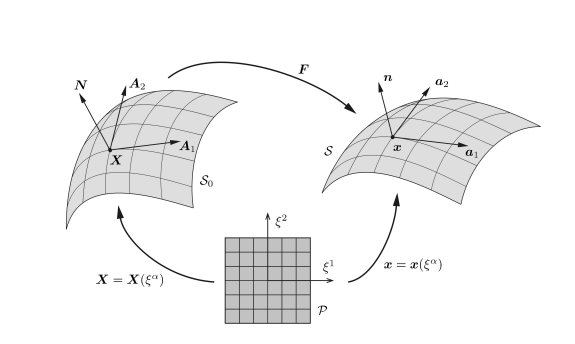
\includegraphics[scale = 0.60]{Images/curvilinear_map.png}
    \caption[Configuration and Motion of a Continuum Surface in Curvilinear Coordinates]{Configuration and motion of a continuum surface in curvilinear coordinates (Image Source: \cite{sauer2014}).}
    \label{fig:curvi_config}
\end{figure}
The membrane surface, denoted $\mathcal{S}$, is fully characterised by 
 the parametric description,
 \begin{equation} \label{parametric_definition}
    \boldsymbol{x} = \boldsymbol{x}(\xi^{1}, \xi^{2}) \, .
 \end{equation}
This is the mappinng of the point $(\xi^{1}, \xi^{2})$ in the parameter domain $\mathcal{P}$
 to the material point $\boldsymbol{x} \in \mathcal{S}$.
According to the non-standard tensor notation used in continuum mechanics,
 Greek indices take on the values 1 and 2 on the surface. And as in the previous section,
 lower case Latin indices take the values 1, 2, and 3, in Euclidean space and summation is
 implied on repeated indices.
The tangent vectors that form the basis at a coordinate $\xi^{\alpha}$ at point $\boldsymbol{x} \in \mathcal{S}$ are
 given by,
 \begin{equation}\label{tangent_parametric}
    \boldsymbol{a}_{\alpha} = \frac{\partial \boldsymbol{x}}{\partial \xi^{\alpha}}, \,\,\, \alpha = 1, 2
 \end{equation}
In general, they are not orthonomal. This basis is thus characterised by the \emph{first fundamental form} of the surface known as the covariant metric tensor,
\begin{equation}\label{metric_def}
    a_{\alpha \beta} := \boldsymbol{a}_{\alpha} \cdot \boldsymbol{a}_{\beta}.
\end{equation}
In case of an orthonormal basis system, the covariant metric tensor reduces to the identity tensor. The contravariant components of the metric tensor can be obtained by its inversion as
\begin{equation}\label{contravar_metric_def}
    [a^{\alpha \beta}] := [a_{\alpha \beta}]^{-1}.
\end{equation}
This enables the construction of a dual basis - the contra-variant counterparts of the covariant base vectors, $\boldsymbol{a}_{\alpha}$,
\begin{align}\label{contravar_def}
    \boldsymbol{a}^{\alpha} &:= a^{\alpha \beta} \boldsymbol{a}_{\beta},\\
    \boldsymbol{a}^{\alpha} &\cdot \boldsymbol{a}^{\beta} = a^{\alpha \beta},\\
    \boldsymbol{a}_{\alpha} &\cdot \boldsymbol{a}^{\beta} = \delta^{\beta}_{\alpha},
\end{align}
where $\delta^{\beta}_{\alpha}$ is the Kronecker delta.
%
The unit normal at a point $\boldsymbol{x} \in \mathcal{S}$ is defined by,
\begin{equation}\label{normal}
    \boldsymbol{n} = \frac{\boldsymbol{a}_{1} \times \boldsymbol{a}_{2}}{\| \boldsymbol{a}_{1} \times \boldsymbol{a}_{2} \|}
    = \frac{\boldsymbol{a}_{1} \times \boldsymbol{a}_{2}}{\sqrt{\det a_{\alpha \beta}}}.
\end{equation}

Any vector, $\boldsymbol{v}$ on $\mathcal{S}$ can thus be decomposed using the covariant or the contravariant basis,
\begin{equation}
    \boldsymbol{v} = v^{\alpha} \boldsymbol{a}_{\alpha} + v_{\mathrm{n}}\boldsymbol{n} = v_{\alpha} \boldsymbol{a}^{\alpha} + v_{\mathrm{n}}\boldsymbol{n},
\end{equation}
 where $v_{\alpha}$ and $v^{\alpha}$ denote the covariant and the contravariant components of the vector respectively.
The derivative and the co-variant derivative of the tangent vectors, $\boldsymbol{a}_{\alpha}$, can be defined as,
\begin{align}\label{tangent_derivatives}
    \boldsymbol{a}_{\alpha , \beta} &= \frac{\partial \boldsymbol{a}_{\alpha}}{\partial \xi^{\beta}},\\
    \boldsymbol{a}_{\alpha ; \beta} := \boldsymbol{a}_{\alpha , \beta} - &(\boldsymbol{a}_{\alpha , \beta} \cdot \boldsymbol{a}^{\gamma}) \boldsymbol{a}_{\gamma} = \boldsymbol{a}_{\alpha , \beta} - \Gamma^{\gamma}_{\alpha \beta} \boldsymbol{a}_{\gamma},
\end{align}
where $\Gamma^{\gamma}_{\alpha \beta}$ are the Christoffel symbols of the second kind.
Defining the identity tensor on the surface, $\mathcal{S}$,
\begin{equation}\label{surface_identity}
    \boldsymbol{1} = \boldsymbol{a}_{\alpha} \otimes \boldsymbol{a}^{\alpha} = \boldsymbol{a}^{\alpha} \otimes \boldsymbol{a}_{\alpha} = \boldsymbol{\tilde{1}} - \boldsymbol{n} \otimes \boldsymbol{n}, 
\end{equation}
where $\boldsymbol{\tilde{1}}$ is the usual identity tensor in $\mathbb{R}^{3}$, two results can be derived.
\begin{equation}\label{con_tgnt}
    \boldsymbol{a}_{\alpha ; \beta} = (\boldsymbol{n} \otimes \boldsymbol{n}) \boldsymbol{a}_{\alpha,\beta}.
\end{equation}
The \emph{second fundamental form} of the surface relates the change in the direction of the normal vector to the surface as the parametric coordinates are varied.
This is known as the curvature tensor with covariant components \footnote{The proofs to \eqref{con_tgnt} and \eqref{curvature_tensor_def} can be found in the appendix, \eqref{appendices:cov_tangent_derivative} and \eqref{appendices:curvature_tensor_derivation}.}
 $\boldsymbol{b} = b_{\alpha \beta} \boldsymbol{a}^{\alpha} \otimes \boldsymbol{a}^{\beta}$, where
\begin{equation} \label{curvature_tensor_def}
    b_{\alpha \beta} := \boldsymbol{n} \cdot \boldsymbol{a}_{\alpha ; \beta} = \boldsymbol{n} \cdot \boldsymbol{a}_{\alpha,\beta}.
\end{equation}
\section{Kinematics}
%---------------------------------------------------------------------------------
As defined in Section \ref{sec:continuum_kinematics}, to consider the deformation of the membrane surface, we distinguish between the reference configuration,
 $\mathcal{S}_{0}$, and the current configuration, $\mathcal{S}$. To describe quantities on $\mathcal{S}$,
 are written in lowercase symbols - $\boldsymbol{x}, \boldsymbol{a}_{\alpha}, \boldsymbol{a}^{\alpha}, \boldsymbol{n}, a_{\alpha \beta}, b_{\alpha \beta}$.
 Correspondingly, uppercase symbols are used to describe the quantities on $\mathcal{S}_{0}$.
 The deformation of a line element in $\mathcal{S}_{0}$ can be described using the Deformation tensor,
\begin{equation}\label{curvy_F}
    \begin{split}
    \mathrm{d}\boldsymbol{x} &= {\boldsymbol{a}_{\alpha} \otimes \boldsymbol{A}^{\alpha}} \mathrm{d} \boldsymbol{X},\\
    &\text{where } \mathrm{d} \boldsymbol{X} = \frac{\partial \boldsymbol{X}}{\partial \xi^{\alpha}} = \boldsymbol{A}_{\alpha} \mathrm{d} \xi^{\alpha}, \notag\\
    &\text{and } \mathrm{d} \boldsymbol{x} = \boldsymbol{a}_{\alpha} \mathrm{d} \xi^{\alpha}. \notag
\end{split}
\end{equation}
The following transformations can be described using \textbf{F},
\begin{align}\label{a_and_A}
    \boldsymbol{a}_{\alpha} &= \left(\boldsymbol{a}_{\alpha} \otimes \boldsymbol{A}^{\alpha}\right) \boldsymbol{A}_{\alpha} = \boldsymbol{FA}_{\alpha},  &  \boldsymbol{a}^{\alpha} &= \left(\boldsymbol{a}^{\alpha} \otimes \boldsymbol{A}_{\alpha}\right) \boldsymbol{A}^{\alpha} = \boldsymbol{F}^{-T} \boldsymbol{A}^{\alpha},\\
    \boldsymbol{A}_{\alpha} &= \left(\boldsymbol{A}_{\alpha} \otimes \boldsymbol{a}^{\alpha}\right) \boldsymbol{a}_{\alpha} = \boldsymbol{F}^{-1} \boldsymbol{a}_{\alpha},  &   \boldsymbol{A}^{\alpha} &= \left(\boldsymbol{A}^{\alpha} \otimes \boldsymbol{a}_{\alpha}\right) \boldsymbol{a}^{\alpha} = \boldsymbol{F}^{T} \boldsymbol{a}^{\alpha}.
\end{align}
The right and left Cauchy-Green surface tensors are,
\begin{align}\label{curvy_strain}
    \boldsymbol{C} &= \boldsymbol{F}^{T} \boldsymbol{F} = a_{\alpha \beta} \boldsymbol{A}^{\alpha} \otimes \boldsymbol{A}^{\beta},   &   \boldsymbol{C}^{-1} &= (\boldsymbol{F}^{T} \boldsymbol{F})^{-1} = a^{\alpha \beta} \boldsymbol{A}_{\alpha} \otimes \boldsymbol{A}_{\beta},\\
    \boldsymbol{b} &= \boldsymbol{F} \boldsymbol{F}^{T} = A^{\alpha \beta} \boldsymbol{a}_{\alpha} \otimes \boldsymbol{a}_{\beta},  &   \boldsymbol{b}^{-1} &= (\boldsymbol{F} \boldsymbol{F}^{T})^{-1} = A_{\alpha \beta} \boldsymbol{a}^{\alpha} \otimes \boldsymbol{a}^{\beta}.
\end{align}

Similar to Section \ref{sec:continuum_kinematics}, the area elements on the surfaces can be related to each other
 with the help of the parametric coordinates $(\xi^{1}, \xi^{2})$. The differential surface area in the current and reference configuration and their relation can be given as,
 \begin{gather} \label{area_something_man}
    \mathrm{d}a := \Vert (\boldsymbol{a}_{1} \mathrm{d}\xi^{1}) \times ((\boldsymbol{a}_{2} \mathrm{d}\xi^{2})) \Vert = \Vert \boldsymbol{a}_{1} \times \boldsymbol{a}_{2} \Vert\, \mathrm{d}\square = \sqrt{\det a_{\alpha \beta}}\,\, \mathrm{d}\square =: J_{a} \mathrm{d}\square,\\
    \mathrm{d}A := \Vert \boldsymbol{A}_{1} \times \boldsymbol{A}_{2} \Vert \, \mathrm{d}\square = \sqrt{\det A_{\alpha \beta}}\,\, \mathrm{d}\square =: J_{A} \mathrm{d}\square.\\    
\end{gather}
where $\mathrm{d} \square := \mathrm{d} \xi^{1} \, \mathrm{d} \xi^{2}$. Using the above defined quantities, 
\begin{equation} \label{area_something_final}
    \mathrm{d}a = \frac{J_{a}}{J_{A}} \mathrm{d}A =: J \mathrm{d}A.
\end{equation} 
 
\section{Momentum Balance}
%---------------------------------------------------------------------------------
At any given point, the Cauchy stress tensor $\boldsymbol{\sigma}$ can be written as,
\begin{equation}\label{curvy_stress}
    \boldsymbol{\sigma} = \sigma^{\alpha \beta} \boldsymbol{a}_{\alpha} \otimes \boldsymbol{a}_{\beta} + \sigma^{3\alpha}(\boldsymbol{n}
    \otimes \boldsymbol{a}_{\alpha} + \boldsymbol{a}_{\alpha} \otimes \boldsymbol{n}) + \sigma^{33} \boldsymbol{n} \otimes \boldsymbol{n}.
\end{equation}
As can be seen from \eqref{curvy_stress}, $\boldsymbol{\sigma}$ is symmetric in this formulation. For membranes, it can be assumed that $\sigma^{3\alpha} = \sigma^{33} = 0$,
 which reduces the stress tensor to the \emph{in-plane Cauchy stress tensor}
\begin{equation}\label{curvy_planar_stress}
    \boldsymbol{\sigma} = \sigma^{\alpha \beta} \boldsymbol{a}_{\alpha} \otimes \boldsymbol{a}_{\beta}.
\end{equation}
From the in-plane Cauchy tensor, the internal traction acting on the surface perpendicular to $\boldsymbol{a}^{\alpha}$ can be written as\footnote{The proof to \eqref{traction_def} can be found in the appendix},
\begin{equation}\label{traction_def}
    \boldsymbol{t}^{\alpha} = \boldsymbol{\sigma} \boldsymbol{a}^{\alpha} = \sigma^{\beta \alpha} \boldsymbol{a}_{\beta},
\end{equation}
Given a distributed surface force \textbf{f},
\begin{equation}\label{surface_force}
    \boldsymbol{f} = f_{\alpha} \boldsymbol{a}^{\alpha} + p \boldsymbol{n} = f^{\alpha} \boldsymbol{a}_{\alpha} + p \boldsymbol{n}.
\end{equation}
the balance of linear momentum in its strong form is \cite{steigmann1999},
\begin{equation}\label{lin_momentum_curvy}
    \boldsymbol{t}^{\alpha}_{;\alpha} + \boldsymbol{f} = \boldsymbol{0}.\
\end{equation}
Using \eqref{traction_def} and \eqref{curvature_tensor_def}, it can be derived that the covariant derivative of $\boldsymbol{t}^{\alpha}$ can be written as
\begin{equation} \label{traction_cov_derivative}
    \boldsymbol{t}^{\alpha}_{;\alpha} = \sigma ^{\beta \alpha}_{;\alpha}\boldsymbol{a}_{\beta} + \sigma^{\beta \alpha} b_{\beta \alpha} \boldsymbol{n}.
\end{equation}
This enables the decomposition of \eqref{lin_momentum_curvy} into an equation for in-plane and out-of-plane equilibrium.
\begin{equation}\label{lin_momentum_curvy_decomposition}
    \begin{cases}
        \sigma^{\beta \alpha}_{;\alpha} + f^{\beta} = 0 \,\,\, \text{(in-plane)}\\
        \sigma^{\beta \alpha} b_{\beta \alpha} + p = 0 \, \, \, \text{(out-of-plane)}
    \end{cases}
\end{equation}
\linebreak
\section{Weak Form} \label{sec:curvy_weak_form}
With the help of a mathematically admissible test function $\boldsymbol{w}$ on $\mathcal{S}$, to derive the weak form \eqref{lin_momentum_curvy} can be written as  
\begin{equation}\label{weak_form_1}
    \int_{\mathcal{S}} \boldsymbol{w} \left[ \boldsymbol{t}_{; \alpha}^{\alpha} + \boldsymbol{f} \right] \, \mathrm{d} a = 0.
\end{equation}
Decomposing $\boldsymbol{w}$ into its surface and normal components     
\begin{equation}\label{weak_form_2}
    0 = \int_{\mathcal{S}} \left[ w_{\gamma} \boldsymbol{a}^{\gamma} + w \boldsymbol{n} \right] \left[ \sigma_{~~; \alpha}^{\beta \alpha} \boldsymbol{a}_{\beta} + \sigma^{\beta \alpha} b_{\beta \alpha} \boldsymbol{n} + \boldsymbol{f} \right] \, \mathrm{d} a
\end{equation}
and using $ \boldsymbol{t} = m_{\alpha} \boldsymbol{t}^{\alpha} = m_{\alpha} \sigma^{\beta \alpha} \boldsymbol{a}_{\beta} $,
 the weak form can be written as \footnote{The complete derivation can be found in the Appendix \ref{appendices:weak_form_derivation}}  
    \begin{equation}\label{weak_form_curvy}
    0 = \int_{\partial \mathcal{S}} w_{\gamma} \overline{t}^{\gamma} \, \mathrm{d} s - \int_{\mathcal{S}} w_{\gamma ; \alpha} \sigma^{\gamma \alpha} \, \mathrm{d} a + \int_{\mathcal{S}} w_{\gamma} f^{\gamma} \, \mathrm{d} a + \int_{\mathcal{S}} w \sigma^{\beta \alpha} b_{\beta \alpha} \, \mathrm{d} a + \int_{\mathcal{S}} w p \, \mathrm{d} s,
    \end{equation}  
thus making it possible to write
    \begin{equation}\label{eq:weak_8}
        G_{int} - G_{ext} = 0 \quad \forall \boldsymbol{w} \in \mathcal{W}
    \end{equation}
with 
    \begin{equation}\label{curvy_Gint}
        G_{\mathrm{int}} := \int_{\mathcal{S}} w_{\alpha ; \beta} \sigma^{\alpha \beta} \, \mathrm{d} a - \int_{\mathcal{S}} w \sigma^{\alpha \beta} b_{\alpha \beta} \, \mathrm{d} a 
    \end{equation}
    \begin{equation}\label{curvy_Gext}
        G_{\mathrm{ext}} := \int_{\mathcal{S}} w_{\alpha} f^{\alpha} \, \mathrm{d} a + \int_{\partial_{t} \mathcal{S}} w_{\alpha} \overline{t}^{\alpha} \, \mathrm{d} s + \int_{\mathcal{S}} w p \, \mathrm{d} a
    \end{equation}
With~\eqref{appendices:w_ab} it is possible to rewrite~\eqref{curvy_Gint} as
    \begin{equation}\label{eq:weak_11}
    G_{\mathrm{int}} = \int_{\mathcal{S}} \boldsymbol{w}_{; \alpha} \cdot \sigma^{\alpha \beta} \boldsymbol{a}_{\beta} \, \mathrm{d} a
    \end{equation}
%---------------------------------------------------------------------------------
%
%
\section{Material Constitution}
For a Neo-Hookean material with a given strain energy density function
\begin{equation}\label{eq:NH_strain}
    W = \frac{\Lambda}{4} \left( J^{2} - 1 - 2 \ln{J} \right) + \frac{\mu}{2} \left( I_{1} - 2 - 2 \ln{J} \right) 
\end{equation}
%
and the traces of the right and left Cauchy-Green tensors in~\eqref{curvy_strain}
\begin{equation}\label{eq:CGtrace}
    I_{1} := \boldsymbol{C} : \boldsymbol{I}_{0} = \boldsymbol{B} : \boldsymbol{I} = a_{\alpha \beta} \boldsymbol{A}^{\alpha} \otimes \boldsymbol{A}^{\beta} : \boldsymbol{A}_{\gamma} \otimes \boldsymbol{A}^{\gamma} = a_{\alpha \beta} \delta^{\alpha}_{\gamma} A^{\beta \delta} = a_{\gamma \beta} A^{\beta \gamma} = a_{\alpha \beta} A^{\alpha \beta}
\end{equation}
the Kirchhoff stress tensor can be written as 
\begin{equation}\label{kirchhoff_stress_def}
        \tau^{\alpha \beta} = 2 \frac{\partial W}{\partial a_{\alpha \beta}} = \left( \frac{\Lambda}{2} \left( J^{2} - 1 \right) - \mu \right) a^{\alpha \beta} - \mu A^{\alpha \beta}.
\end{equation}
Using~\eqref{kirchhoff_stress_def}, the compliance matrix in the current configuration
\begin{equation}\label{curvy_compliance_current_def}
    c^{\alpha \beta \gamma \delta} = \frac{\partial^{2} W}{\partial a_{\alpha \beta} \partial a_{\gamma \delta}} = 2 \frac{\partial \tau^{\alpha \beta}}{\partial a_{\gamma \delta}}
\end{equation}
%
can be written as\footnote{A complete derivation can be found in the Appendix \ref{appendices:compliance_matrix_curvy}}
\begin{equation}\label{curvy_compliance_current}
        c^{\alpha \beta \gamma \delta} = \Lambda J^{2} a^{\alpha \beta} a^{\gamma \delta} + \left( \frac{\Lambda}{2} \left( J^{2} - 1 \right) - \mu \right) m^{\alpha \beta \gamma \delta}.
\end{equation}
where
\begin{equation} \label{mabgd}
    m^{\alpha \beta \gamma \delta} = \frac{1}{a} \left( e^{\alpha \gamma} e^{\delta \beta} + e^{\alpha \delta} e^{\gamma \beta} \right) - 2 a^{\alpha \beta} a^{\gamma \delta}
\end{equation}
%---------------------------------------------------------------------------------
%
\section{Volume Constraint}
The volume enclosed by the membrane $\mathcal{S}$ may be constrained. For the volume enclosed by the reference configuration $V_{0}$
 and the current configuration $V$, this can be defined as
 \begin{equation}\label{vol_constraint_def}
    g_{v} := V_{0} - V = 0.
 \end{equation}
 The enclosed volumes $V$ and $V_{0}$ can be computed with the help of the following surface integrals
 \begin{align} \label{volume_definition}
    V &= \frac{1}{3} \int_{\mathcal{S}} \boldsymbol{x} \cdot \boldsymbol{n} \,\mathrm{d}a, & V_{0} &= \frac{1}{3} \int_{\mathcal{S_{0}}} \boldsymbol{X} \cdot \boldsymbol{N}\,\mathrm{d}A.
 \end{align}
For quasi-static conditions, as is the case for the examples considered in this report,
 the medium enclosed by the membrane can be characterised by pressure and volume. Thus, $g_{v}$ can be applied as a global constraint to the system. 
%---------------------------------------------------------------------------------
%
%
\section{Discretization}
Following the procedures and nomenclature defined in Section \ref{sec:nonlinear_discretisation}, for quadrilateral finite elements $\Omega^{e}_{0}$ and $\Omega^{e}$
 related to a reference element in the parametric space, the discretisations of the nodal variables in the current and the reference configurations are given according to \eqref{nodal_discretisations}.
The tangent vectors~\eqref{tangent_parametric} can be approximated by
\begin{equation} \label{tangent_parametric_discrete}
    \boldsymbol{a}_{\alpha} \approx \sum^{n_{en}}_{I} N_{I,\alpha} \boldsymbol{x}_{I} = \mathbf{N}_{,\alpha} \mathbf{x}_{e}
\end{equation}
where summation is carried out over the $n_{en}$ nodes of the element. The shape function matrix and its derivative with respect to the parametric coordinates
 is given as
\begin{align} \label{curvy_shape_function}
    N &:= \left[N_{1}\boldsymbol{\tilde{1}}, N_{2} \boldsymbol{\tilde{1}},\dots, N_{n_{en}} \boldsymbol{\tilde{1}}\right],\\
    N_{I,\alpha} & = \frac{\partial N_{I}}{\partial \xi^{\alpha}}.
\end{align}
%
Using~\eqref{eq:w_cov}, and~\eqref{tangent_parametric_discrete}, the internal virtual work
 over a finite element is discretised as
 \begin{equation} \label{curvy_Gint_discrete}
    \begin{split}
    G^{e}_{\text{int}} = \int_{\Omega_{0}^{e}} \boldsymbol{w}_{;\alpha} \cdot \tau^{\alpha \beta} \boldsymbol{a}_{\beta} \,dA 
    &\approx \mathbf{w}^{T}_{e} \int_{\Omega_{0}^{e}} \mathbf{N}^T_{,\alpha} \tau^{\alpha \beta} \mathbf{N}_{,\beta}\,dA \,\, \mathbf{x}_{e}\\ & =: \mathbf{w}^{T}_{e} \mathbf{f}^{e}_{int}.
    \end{split}
 \end{equation}
The internal virtual work~\eqref{curvy_Gint} can further be decomposed and discretised into its in-plane and out-of-plane components
 using~\eqref{eq:w_alp_cov} and the discretisation of the curvature tensor in order to obtain the corresponding force vectors, $\mathbf{f}^{e}_{\text{inti}}$
 and $\mathbf{f}^{e}_{\text{into}}$
\begin{align} \label{curvy_Gint_decomposed_discretised}
    G_{\text{inti}}^{e} &= \int_{\Omega_{0}} w_{\alpha;\beta} \tau^{\alpha \beta}\,dA \approx \mathbf{w}_{e}^{T} \mathbf{f}^{e}_{\text{inti}} = \mathbf{w}_{e}^{T} \int_{\Omega_{0}^{e}} \tau^{\alpha \beta}
    \left[ \mathbf{N}_{, \alpha}^{T} \mathbf{N}_{, \beta} + \mathbf{N}^{T} \left( \boldsymbol{n} \otimes \boldsymbol{n} \right) \mathbf{N}_{, \alpha \beta} \right]\,dA \mathbf{x}_{e},\\
    G_{\text{into}}^{e} &= -\int_{\Omega_{0}^{e}} w \tau^{\alpha \beta} b_{\alpha \beta}\,dA 
    \approx \mathbf{w}_{e}^{T} \mathbf{f}^{e}_{\text{into}} = - \mathbf{w}_{e}^{T}\int_{\Omega_{0}^{e}} \tau^{\alpha \beta}\mathbf{N}^{T} \left( \boldsymbol{n} \otimes \boldsymbol{n} \right) \mathbf{N}_{, \alpha \beta}\,dA \mathbf{x}_{e}.
\end{align}
The external virtual work~\eqref{curvy_Gext} can be discretised to yield the external force vector $\mathbf{f}^{e}_{\text{ext}}$, 
\begin{equation}\label{curvy_Gext_discretised}
    \begin{split}
        G_{\text{ext}}^{e} &= \int_{\Omega_{0}^{e}} \boldsymbol{w} \cdot \boldsymbol{f}_{0}\,dA + \int_{\partial_{t}\Omega^{e}} \boldsymbol{w}\cdot \overline{\boldsymbol{t}}\,ds + \int_{\Omega^{e}} wp \,da,\\
        &\approx \mathbf{w}^{T}_{e} \left(\int_{\Omega_{0}^{e}} \mathbf{N}^{t} \boldsymbol{f}_{0} \,dA + \int_{\partial_{t} \Omega^{e}} \mathbf{N}^{T} \overline{\boldsymbol{t}}\,ds + \int_{\Omega^{e}} \mathbf{N}^{T} p \boldsymbol{n} \,da \right) =: \mathbf{w}^{T}_{e} \mathbf{f}^{e}_{\text{ext}}.
    \end{split}
\end{equation}
In~\eqref{curvy_Gext_discretised}, the external loading is assumed to be of the form $\boldsymbol{f} = \boldsymbol{f}_{0}/J + p\boldsymbol{n}$, where $\boldsymbol{f}_{0}$ and $p$ are the specified loading parameters. 
Using \eqref{curvy_Gint_discrete} and \eqref{curvy_Gext_discretised}, the discretised weak form can be written as
\begin{equation} \label{curvy_weak_form_discretised}
    \mathbf{w}^{T}\left[\mathbf{f}^{e}_{\text{int}} - \mathbf{f}^{e}_{\text{ext}}\right] = \boldsymbol{0}.
\end{equation}
Since the discretised test functions $\mathbf{w}$ are arbitrary and zero on the Dirichlet boundary, the system of discretised nonlinear equilibrium equations
 to be solved for the unknown nodal positions $\mathbf{x}$ is
 \begin{equation} \label{curvy_f_system}
    \mathbf{f}\left(\mathbf{x}, p\right) := \mathbf{f}_{\text{int}} - \mathbf{f}_{\text{ext}} = \boldsymbol{0}.
 \end{equation} 
For the volume constraint \eqref{vol_constraint_def}, $V_{0}$ can be prescribed externally, thus the discretisation of $V$ is sufficient
 for the discretisation of $g_{v}$. The volume enclosed by the discretised membrane surface can be given as
 \begin{equation} \label{discretised_volume_constraint}
    \mathrm{V} = \sum_{e=1}^{n_{el}} \mathrm{V}^{e} = \frac{1}{3} \sum_{e=1}^{n_{el}} \int_{\Omega^{e}} \boldsymbol{n}^{T} \mathbf{N}\,\mathrm{d}a \mathbf{x}_{e}.
 \end{equation}
Volume constraints are included in the formulation with the help of the Lagrange multiplier method. The multiplier associated
 with the constrain in this case is the pressure $p$ acting on the membrane[Sauer 2014]. In this case, the nonlinear system of equations \eqref{curvy_f_system} is given as
 \begin{align} \label{curvy_f_constrained}
    \mathbf{f}\left(\mathbf{x}, p\right) &= \boldsymbol{0},\\
    g_{v} \left(\mathbf{x}\right) &= 0,
 \end{align}
 that needs to be solved for the unknown nodal positions $\mathbf{x}$ and pressure $p$. 

%-----------------------------------------------------------------------------------
%
%
\section{Linearization}
As in Section \ref{sec:newton_raphson_lin}, due to the existent nonlinearities in the system \eqref{curvy_f_system} will be solved using Newton's method. 
 This requires consistent linearisation of the discrete system with respect to the variables involved. 
 The derivations of linearised quantities required to formulate $\Delta \mathbf{f}_{\text{int}}^{e}$ and $\Delta \mathbf{f}_{\text{ext}}^{e}$ can be found in the Appendix \ref{appendices:curvy_linearisations}.
 The linearisation of $\mathbf{f}_{\text{int}}$ with respect to $\mathbf{x}$ at the element level can be given as
\begin{equation}\label{eq:del_fint_def}
    \begin{split}
        \Delta \mathbf{f}_{\mathrm{int}}^{e} &= \int_{\Omega^{e}} \Delta \left[\mathbf{N}^{T}_{, \alpha} \tau^{\alpha \beta} \mathbf{N}_{, \beta} \, \mathbf{x}_{e}\right] \mathrm{d} A\\ 
        &= \underbrace{\int_{\Omega^{e}} c^{\alpha \beta \gamma \delta} \mathbf{N}_{, \alpha}^{T} \left( \boldsymbol{a}_{\beta} \otimes \boldsymbol{a}_{\gamma} \right) \mathbf{N}_{, \delta} \, \mathrm{d} A}_{=: k_{\mathrm{mat}}^{e}} \,\Delta \mathbf{x}_{e} + \underbrace{\int_{\Omega^{e}} \mathbf{N}_{,\alpha}^{T} \tau^{\alpha \beta} \mathbf{N}_{, \beta} \, \mathrm{d} A}_{=: k_{\mathrm{geo}}^{e}} \,\Delta \mathbf{x}_{e}.
    \end{split}
\end{equation}
The two contributions can be split into the tangent matrices associated with the internal virtual work - the \emph{material} and the \emph{geometric stiffness matrix} such that
\begin{equation}\label{eq:del_f_int_3}
\Delta \mathbf{f}_{\mathrm{int}}^{e} = \left(\mathbf{k}_{\text{mat}}^{e} + \mathbf{k}_{\text{geo}}^{e} \right) \Delta \mathbf{x}_{e}.
\end{equation}
For dead loading, the external force vector at the element level $\mathbf{f}_{\text{ext}}^{e}$ defined in \eqref{curvy_Gext_discretised} can be reduced to
\begin{equation}\label{eq:f_ext_dead}
\mathbf{f}_{\mathrm{ext}}^{e} = \int_{\Omega^{e}} \mathbf{N}^{T} p \boldsymbol{n} \, \mathrm{d} a.
\end{equation}
The reduced external force vector linearised with respect to $\mathbf{x}$ and the pressure $p$ is given as
\begin{equation}\label{eq:del_f_ext_dead_def}
    \begin{split}
        \Delta \mathbf{f}_{\mathrm{ext}}^{e} &= \int_{\Omega^{e}} \rho \mathbf{N}^{T} \left( \boldsymbol{n} \otimes \boldsymbol{g} \right) \, \mathrm{d} a \Delta \mathbf{x}_{e} + \int_{\Omega^{e}} p \mathbf{N}^{T} \left( \boldsymbol{n} \otimes \boldsymbol{a}^{\alpha} - \boldsymbol{a}^{\alpha} \otimes \boldsymbol{n} \right) \mathbf{N}_{, \alpha} \, \mathrm{d} a \Delta \mathbf{x}_{e}\\
        &=: \mathbf{k}_{\text{ext}}^{e} \Delta \mathbf{x}_{e},
    \end{split}
\end{equation}
where the tangent matrix associated with the external virtual work is $\mathbf{k}_{\text{ext}}^{e}$.
At the element level, the linearisation of $g_{v}^{e}$ can be given as
\begin{equation} \label{lin_vol_constraint}
    \begin{split}
        \Delta g_{v}^{e} &= \Delta V_{0} - \frac{1}{3} \Delta \left[\int_{\Omega^{e}} \boldsymbol{n}^{T} \mathbf{N} \,\mathrm{d} a \mathbf{x}_{e}\right]\\
                        &= 0 - \frac{1}{3}\int_{\Omega^{e}}\boldsymbol{n}^{T} \mathbf{N} \,\mathrm{d}a \Delta \mathbf{x}_{e}
                        - \frac{1}{3} \int_{\Omega^{e}} \boldsymbol{x} \cdot \left(\boldsymbol{n} \otimes \boldsymbol{a}^{\alpha} - \boldsymbol{a}^{\alpha} \otimes \boldsymbol{n}\right)\mathbf{n}_{,\alpha}\, \mathrm{d}a \Delta \boldsymbol{x}_{e}\\
                        &:= \mathbf{h}_{v}^{e} \Delta \mathbf{x}_{e}.
    \end{split}
\end{equation}
When volume constraints are applicable, the internal pressure $p_{v}$ acts as the unknown Lagrange multiplier and needs to be accounted for.
Thus, the linearised external force vector with the constraint is given as
\begin{equation} \label{del_f_ext_const}
    \Delta \mathbf{f}_{\text{ext}}^{e} = \mathbf{k}_{\text{ext}}^{e} \Delta \mathbf{x}_{e} + \mathbf{l}^{e}_{\text{ext}} \Delta p_{v},
\end{equation}
where
\begin{equation}
    \mathbf{l}_{\text{ext}}^{e} = \frac{\partial \mathbf{f}_{\text{ext}^{e}}}{\partial p_{v}} = \int_{\Omega^{e}} \mathbf{N}^{T} \boldsymbol{n} \,\mathrm{d}a.
\end{equation}
Using \eqref{eq:del_fint_def}, \eqref{del_f_ext_const}, and \eqref{lin_vol_constraint}, the tangent matrix associated
 with the constrained nonlinear system of equations \eqref{curvy_f_constrained} can be assembled as
 \begin{equation} \label{final_tangent_matrix}
    \mathbf{k}^{e} := \begin{bmatrix}
        \mathbf{k}^{e}_{\text{int}} - \mathbf{k}^{e}_{\text{ext}} & -\mathbf{l}^{e}_{\text{ext}}\\
        \mathbf{h}_{v}^{e} & 0\\
    \end{bmatrix}
\end{equation}
which describes the changes in $\mathbf{f}_{\text{int}} - \mathbf{f}_{\text{ext}}$ and $g_{v}$ due to the changes in $\mathbf{x}_{e}$ and pressure $p_{v}$.

\section{Numerical Examples: Inflation of Square Sheet}
The validation of the framework is undertaken through the consideration of a square sheet with length $\frac{\mathrm{L}}{\mathrm{L}_{0}} = 10$ units and width $\frac{\mathrm{W}}{\mathrm{W}_{0}} = 10$ units respectively under gravitational loading and
 gravitational loading with a volume constraint. An isotropic pre-stretch of $\lambda_{0} = 1.1$ is applied to provide an initial
 out-of-plane stiffness, remove existing instabilites, and the structure is then inflated. The sheet is meshed using standard quadrilateral Lagrangian elements with the additional possibility of h- and p-refinements.
 The real elements are mapped onto a master element onto which the numerical integration is carried out to solve the system of nonlinear equations.
 Figures \ref{fig:mem_grav} and \ref{fig:mem_vol} depict the inflation of the square sheet under gravitational loading and volume constraints respectively with the
 colouring denoting the first invariant of stress. As can be seen, for the case with gravitational loading, increasing values of stress are found at the boundaries
 of the sheet. On the contrary, for the case of loading with a volume contraint, maximum stress is seen at the bottom tip with increasing amounts of deformation. \newline
\begin{figure}[h]
    \centering
    \hspace*{-2.5cm}
    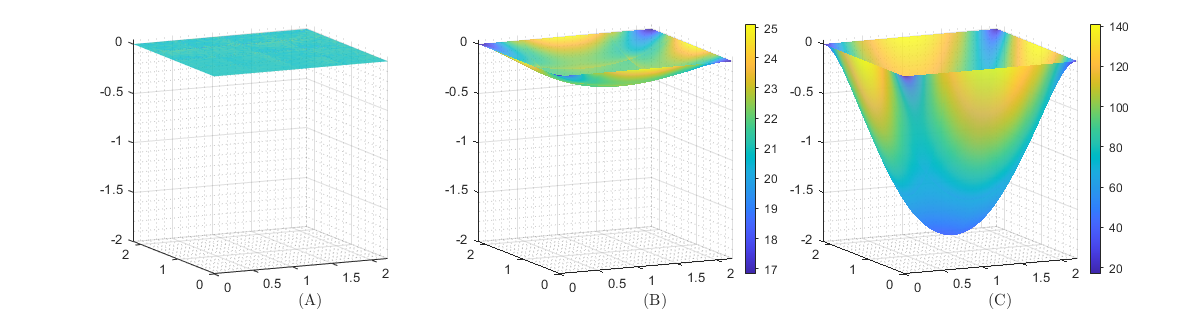
\includegraphics[scale = 0.6]{Images/mem_grav.png}
    \caption[Inflation of Square Sheet under Gravitational Loading]{Inflation of square sheet under gravitational loading: Configurations for $V = \{0, 0.6, 6\} V_{0}$. The colouring denotes the first invariant of stress.}
    \label{fig:mem_grav}
\end{figure}
\noindent Furthermore, the internal pressure is plotted against the enclosed volume in Figure \ref{fig:mem_pres} for various
 orders of approximating polynomials for the case of loading with volume constraint. The significant difference between
 the results of linear Lagrange elements as opposed to the higher-order elements is a result of the higher-order elements
 capturing the shape of the deformed structure more accurately. The relation of internal pressure and enclosed
 volume begins to converge to some solution for quadratic and quintic polynomials. 
\newpage
\begin{figure}[t]
    \centering
    \hspace*{-2cm}
    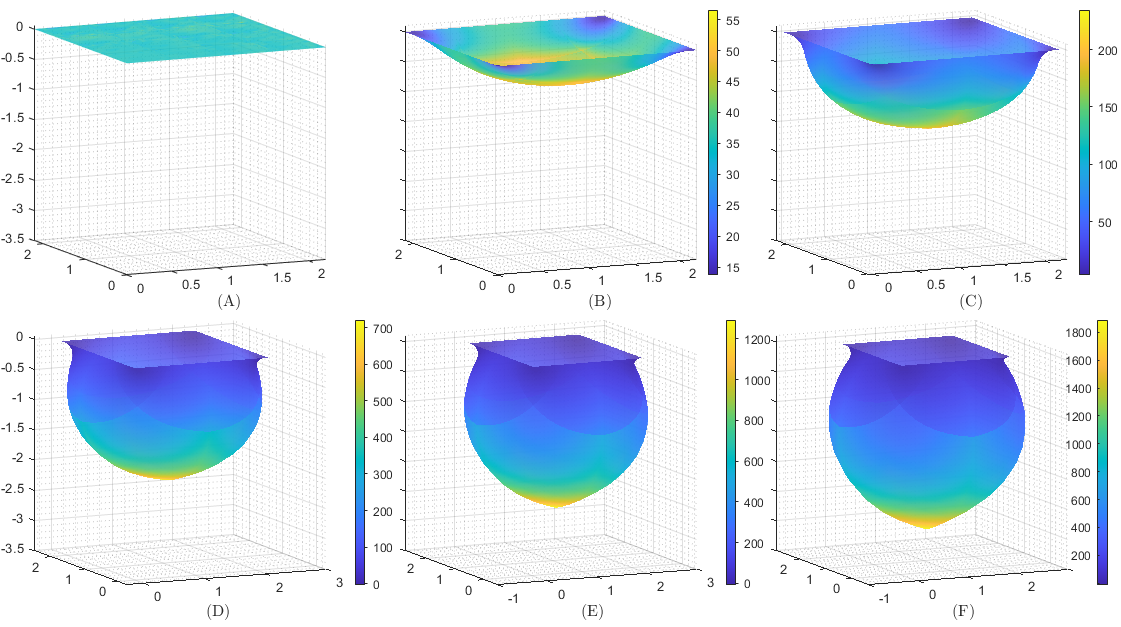
\includegraphics[scale = 0.65]{Images/mem_vol2.png}
    \caption[Inflation of Square Sheet with Volume Constraint]{Inflation of square sheet under loading with volume constraint: Configurations for $V = \{0, 2, 5, 10, 15, 20\} V_{0}$. The colouring denotes the first invariant of stress.}
    \label{fig:mem_vol}
\end{figure}
\begin{wrapfigure}{l}{0.5\textwidth}
    \centering
    \hspace*{-2cm}
    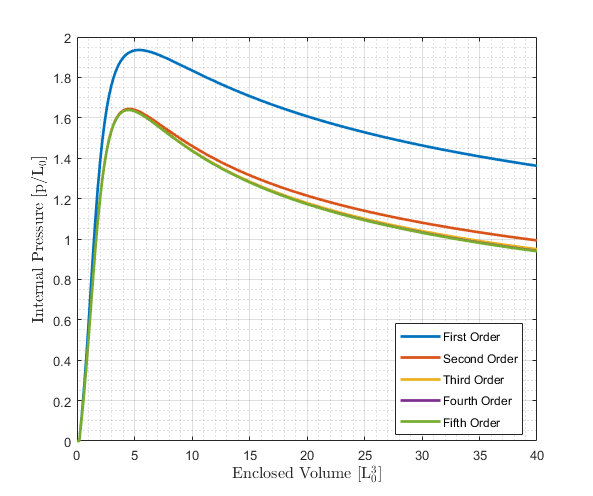
\includegraphics[scale = 0.60]{Images/mem_pres.png}
    \caption[Pressure-Volume Relation for Inflation of Square Sheet for Various Orders of Elements]{Internal pressure against volume for the inflation of square sheet}
    \label{fig:mem_pres}
\end{wrapfigure}
This is seen qualitatively in figure \ref{fig:mem_def} which shows the deformed sheet for a prescribed volume of $V=400V_0$ with 4x4 elements of various
 orders. With increasing order of the used approximation polynomial, the deformed configuration becomes smoother. For quadratic
 and cubic elements, the highest value of the first invariant of the stress tensor is found at a pronounced 'peak' at
 the bottom. Whereas in the quantic elements it disappears altogether, giving a smooth representation of the deformed structure.
 Based on this observation, one can state that the higher-order elements can represent the problem more accurately and closer
 to reality. Further improvements to the current framework can be achieved by using different
 approximation polynomials like isogeometric shape functions as can be seen in \cite{sauer2014}.
 \begin{figure}[h]
    \centering
    \begin{subfigure} [h] {0.48\textwidth}
        \hspace*{-3cm}
        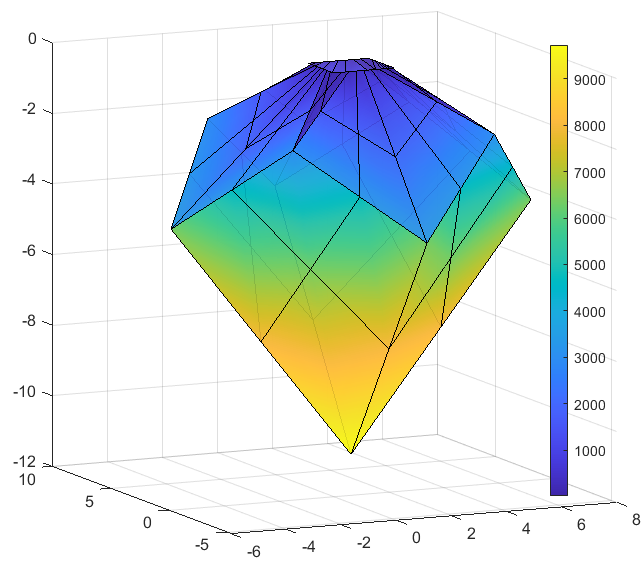
\includegraphics[scale = 0.55]{Images/mem_def1.png}
        \caption[]{4x4 linear elements}
        \label{fig:mem_def1}
    \end{subfigure}
    \hfill
    \begin{subfigure} [h] {0.48\textwidth}
        \hspace*{-.25cm}
        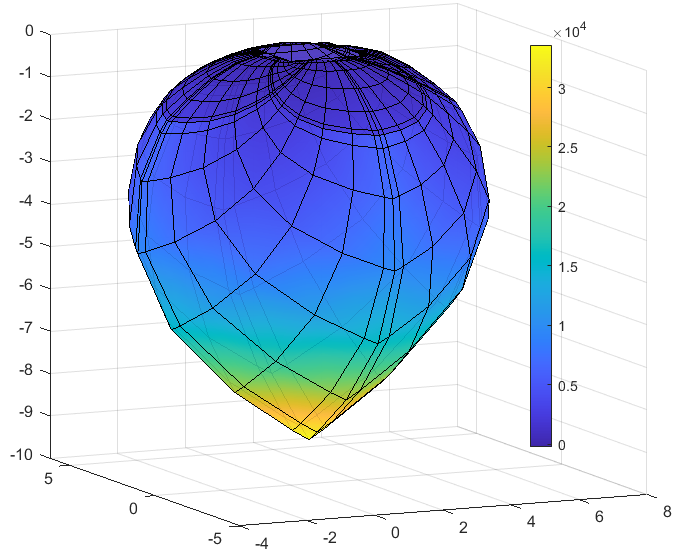
\includegraphics[scale = 0.55]{Images/mem_def2.png}
        \caption[]{4x4 quadratic elements}
        \label{fig:mem_def2}
    \end{subfigure}
    \\
    \begin{subfigure} [h] {0.48\textwidth}
        \hspace*{-3cm}
        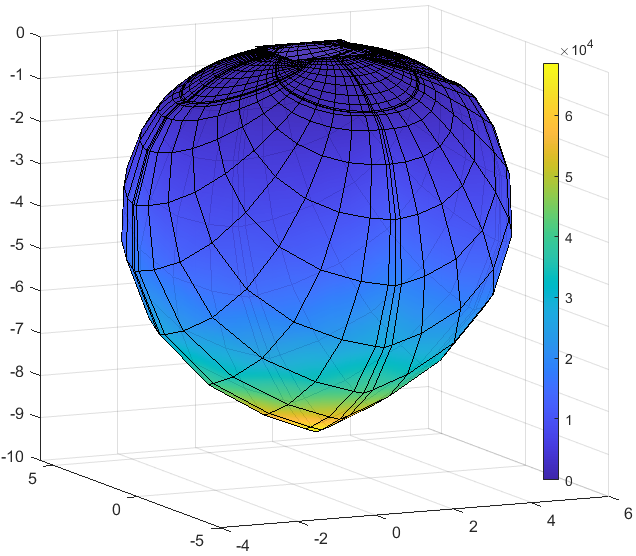
\includegraphics[scale = 0.55]{Images/mem_def3.png}
        \caption[]{4x4 cubic elements}
        \label{fig:mem_def3}
    \end{subfigure}
    \hfill
    \begin{subfigure} [h] {0.48\textwidth}
        \hspace*{-.25cm}
        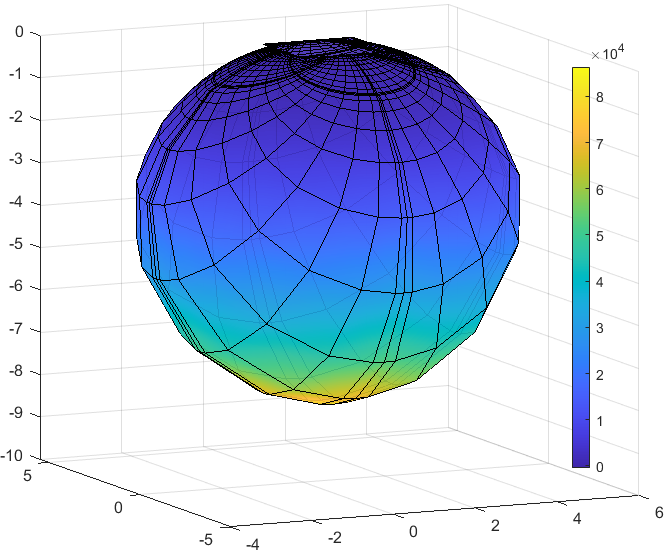
\includegraphics[scale = 0.55]{Images/mem_def5.png}
        \caption[]{4x4 quintic elements}
        \label{fig:mem_def5}
    \end{subfigure}
    \caption[Large Deformation of Square Sheet using Various Orders of Elemets]{Inflated square sheet: $V = 400 V_{0}$}
    \label{fig:mem_def}
\end{figure}


 \afterpage{\blankpage}